% Author: Matthew Turner

\documentclass[11pt,letterpaper]{article}
% \documentclass[11pt]{report}
% \documentclass{report}
% \documentclass{book}
\usepackage[bookmarks]{hyperref}
\usepackage{amssymb,amsmath}
% \usepackage{fullpage}
\usepackage{tabulary}
\usepackage{tabularx}

% \usepackage[margin=1.00in]{geometry}
\usepackage[margin=0.90in]{geometry}
\usepackage{float}

\usepackage{caption}
\usepackage{booktabs}
\usepackage{pslatex}
\usepackage{apacite}
\usepackage{subcaption}
\usepackage{pgfplots}
\usepackage{wrapfig}
\usepackage[english]{babel}
\usepackage{lmodern}
\usepackage{setspace}
\doublespace
% \usepackage{url}
\usepackage{bigfoot}
\usepackage[export]{adjustbox}
\setlength\intextsep{0pt}
\hypersetup{linktocpage}

\usepackage{graphicx}

\title{\vspace{-1in}Identity signaling model progress}

\author{} %{Matthew A.~Turner}}

\begin{document}
\maketitle
\tableofcontents

\section{Evolution in signaling and receiving strategies}

For these preliminary results I focus on the evolution of signaling strategies,
each agent at model initialization. There are two output measures in these experiments:
density of covert signalers and density of churlish receivers. 
There are confirmatory results for two computational experiments in which I: 
(1) varied relative covert receptivity $r/R$ and 
homophily, $w$; and (2) varied the disliking penalties set equal, $d=\delta$,
and homophily, $w$.

The bonus payoff for two 
interacting agents where at least one
likes the other is set fixed to $s=0.25$. The payoff structure is as follows

\begin{table}[H]
  \centering
  \begin{tabular}{rcc}
    Attitude combo. & Payoff (similar) & Payoff (dissim.) \\
   \toprule
    Like/like & $1 + s$                    & NA \\
    Like/neutral & $1 + s$                 & NA \\
    Like/dislike & $1 + s - d$             & NA \\
    Neutral/neutral & 1 + s                & 1  \\
    Dislike/neutral & $1 + s - d$          & $1-d$\\
    Dislike/dislike & $1 + s - d - \delta$ & $1 - d - \delta$
  \end{tabular}
\end{table}

Agents only interact with one another with probability given by their attitudes
towards one another. If two agents are assorted together to potentially 
interact, these are the probabilities the agents do interact.

\begin{table}[H]
  \centering
  \begin{tabular}{rc}
    Attitudes & Pr(paired agents interact) \\
    \toprule
    Like/like & $0.5 + w$ \\
    Like/neutral & $0.5 + \frac{w}{2}$ \\
    Like/dislike & $0.5$ \\
    Neutral/neutral & $0.5$ \\
    Dislike/neutral & $0.5 - \frac{w}{2}$ \\
    Dislike/dislike & $0.5 - w$ 
  \end{tabular}
\end{table}

\subsection{Density of covert signalers vs. $r/R$ and homophily, $w$}

Based on results from ``Evolution of covert signaling'' (``ECS''), I designed
the first agent-based model experiment to determine the dependence of the
density of covert signalers in the population ($\rho_C$) on
the receptiveness of the population to covert signals ($r$) and the
importance of homophily ($w$) to assortment. 

Here I set $R=0.5$, $s=0.25$, $d=\delta=0.25$,
and $N=100$. After signaling, agents go through 10 rounds of assortment/interaction,
followed by evolution after the 10 rounds of interaction. The model has been
run out to 100 timesteps where timeseries are nearly stable, though we will
want more timesteps for our final study, or perhaps adjust the number of 
assortment/interaction rounds up or down per timestep, to guarantee full 
stability.

I systematically varied $r/R$ by setting $R=0.5$ and varied 
$r \in \{0.0, 0.05, 0.1, \ldots, 0.45\}$ to get $r/R \in \{0.0, 0.1, \ldots, 0.9\}$.
I varied homophily identically to $r$, $w \in \{0.0, 0.5, \ldots, 0.45\}$. Note
that both $r$ and $w$ are bounded above by 0.5.

\begin{figure}[H]

  \centering
  \begin{subfigure}{0.49\textwidth}
    \centering
    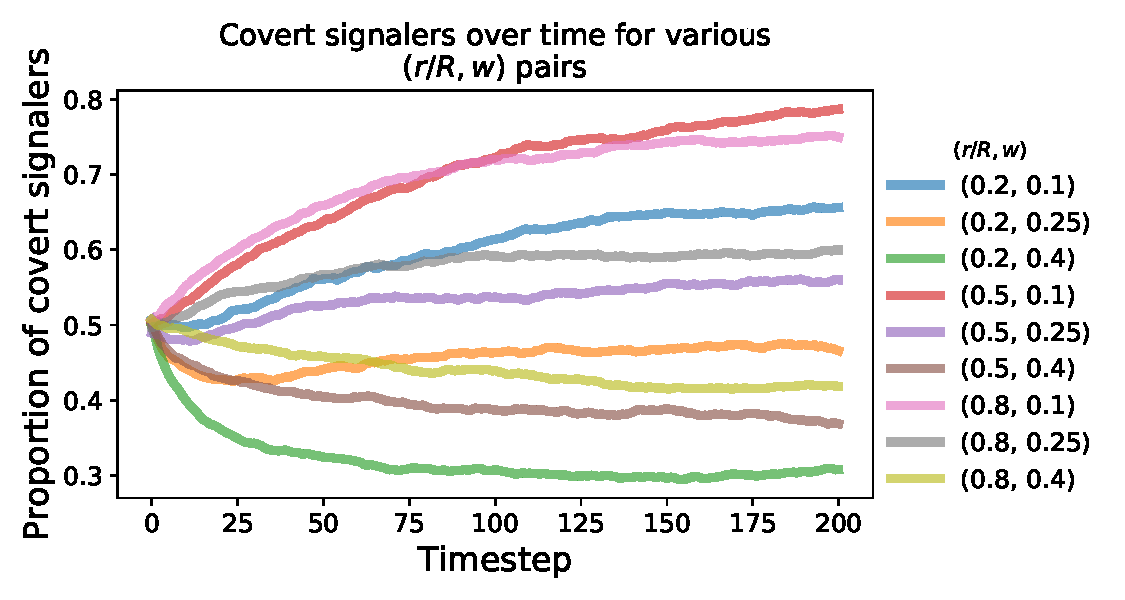
\includegraphics[width=\textwidth]{Figures/receptivityHomophilyCovertSeries.pdf}
    \caption{Density of covert signalers.}
  \end{subfigure}
  \begin{subfigure}{0.49\textwidth}
    \centering
    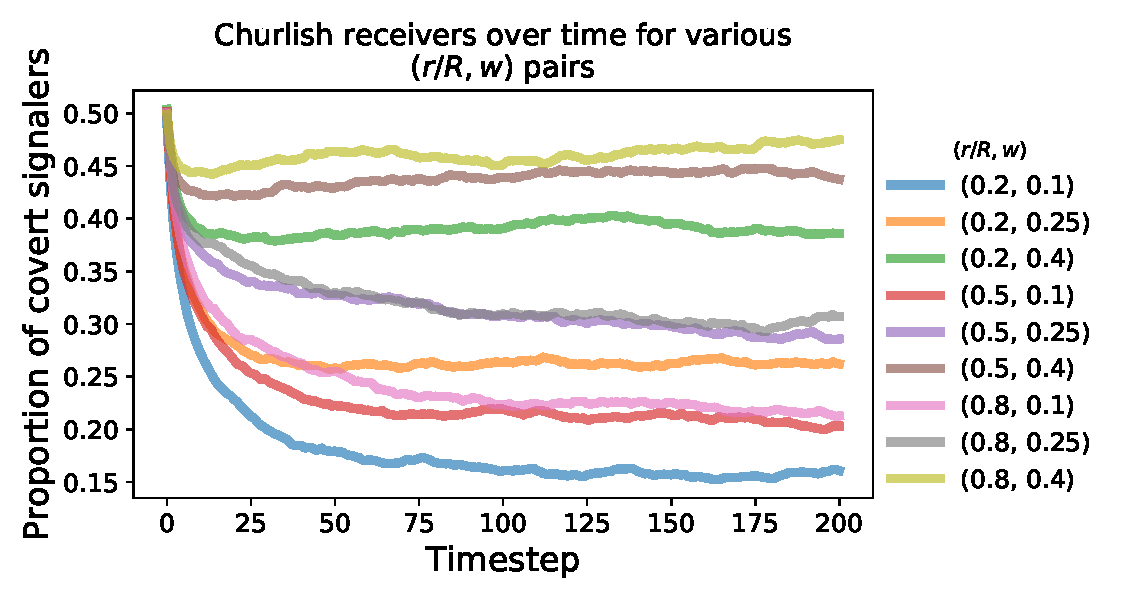
\includegraphics[width=\textwidth]{Figures/receptivityHomophilyChurlishSeries.pdf}
    \caption{Density of churlish receivers.}
  \end{subfigure}
  
  \caption{Timeseries of density of covert signalers and churlish receivers
    for nine combinations of $r$ and $w$. Receptivity of
    overt signals is $R=0.5$.}
  \label{fig:dislikingHomophilySeries}
\end{figure}

\begin{figure}[H]
  \centering
  \begin{subfigure}{0.49\textwidth}
    \centering
    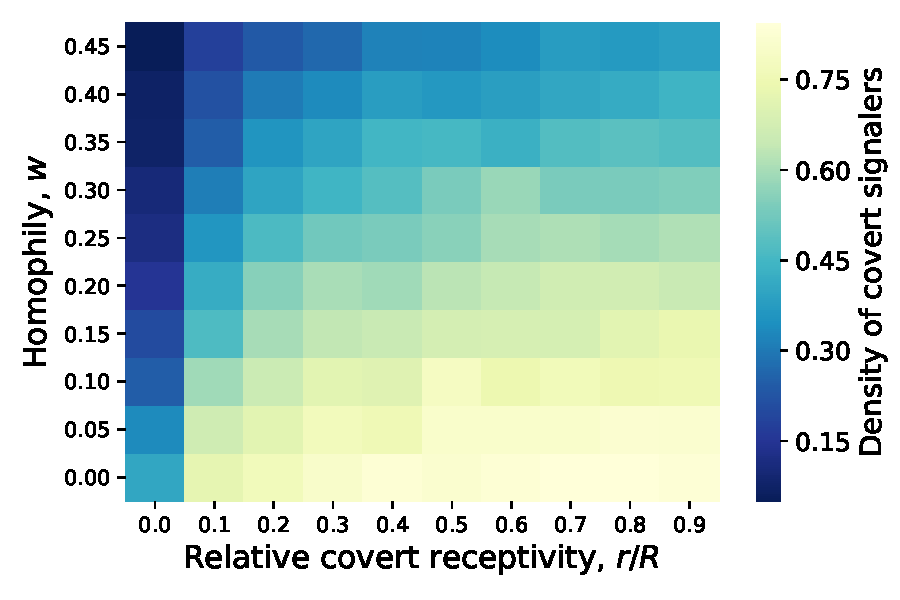
\includegraphics[width=\textwidth]{Figures/covertDensityVsReceptivityHomophilyCoevo.pdf}
    \caption{Density of covert signalers.}
  \end{subfigure}
  \begin{subfigure}{0.49\textwidth}
    \centering
    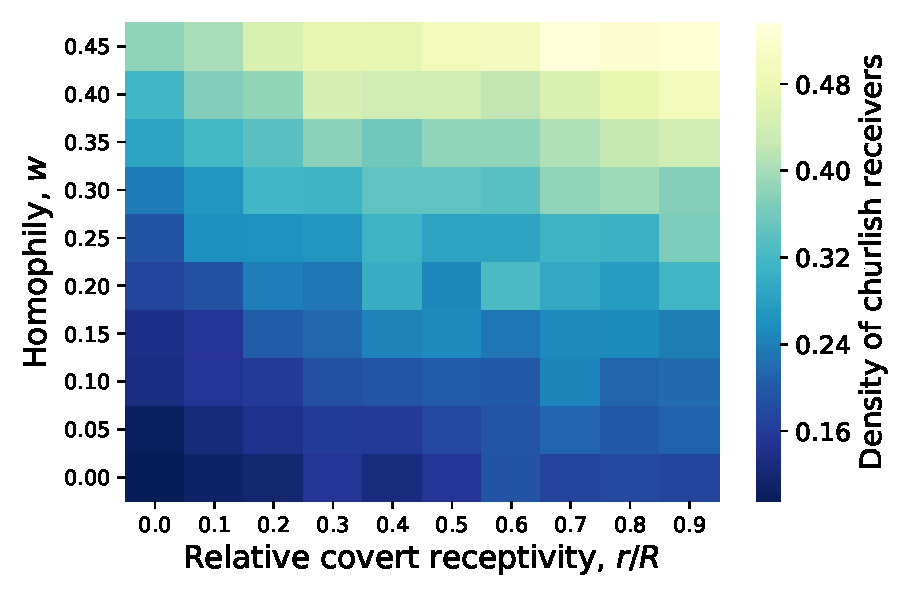
\includegraphics[width=\textwidth]{Figures/churlishDensityVsReceptivityHomophilyCoevo.pdf}
    \caption{Density of churlish receivers.}
  \end{subfigure}
  
  \caption{Density of covert signalers and churlish receivers at $t=200$, 
    final timestep recorded in this preliminary experiment. Receptivity of
    overt signals is $R=0.5$.}
  \label{fig:dislikingHomophilyHeatmap}
\end{figure}


\subsection{Density of covert signalers vs. disliking penalty $d=\delta$ and homophily, $w$}

Here I co-vary the disliking penalties, which I set equal ($d=\delta$), and
homophily, $w$. Here, $r=0.25$ and $R=0.5$. 

Specifically, I vary $d=\delta \in \{0.0, 0.05, 0.1, \ldots, 0.45\}$
As in the above experiment, I set $w \in \{0.0, 0.5, \ldots, 0.45\}$.

\begin{figure}[H]

  \centering
  \begin{subfigure}{0.49\textwidth}
    \centering
    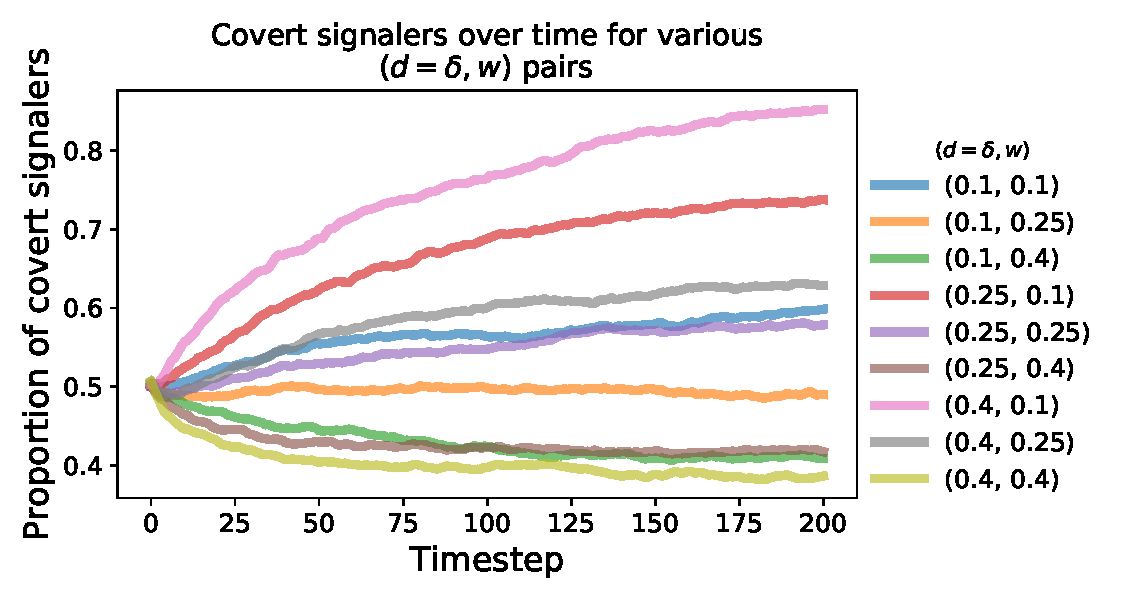
\includegraphics[width=\textwidth]{Figures/dislikingHomophilyCovertSeries.pdf}
    \caption{Density of covert signalers.}
  \end{subfigure}
  \begin{subfigure}{0.49\textwidth}
    \centering
    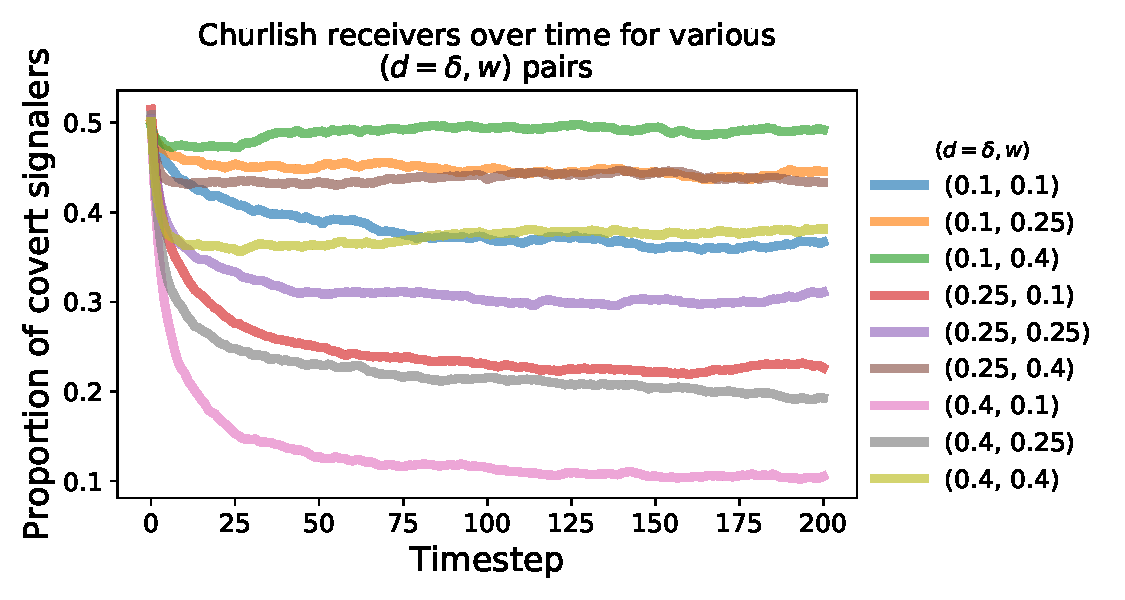
\includegraphics[width=\textwidth]{Figures/dislikingHomophilyChurlishSeries.pdf}
    \caption{Density of churlish receivers.}
  \end{subfigure}
  
  \caption{Timeseries of density of covert signalers and churlish receivers
    for nine combinations of $d=\delta$ and $w$.}
  \label{fig:dislikingHomophilySeries}
\end{figure}

\begin{figure}[H]
  \centering
  \begin{subfigure}{0.49\textwidth}
    \centering
    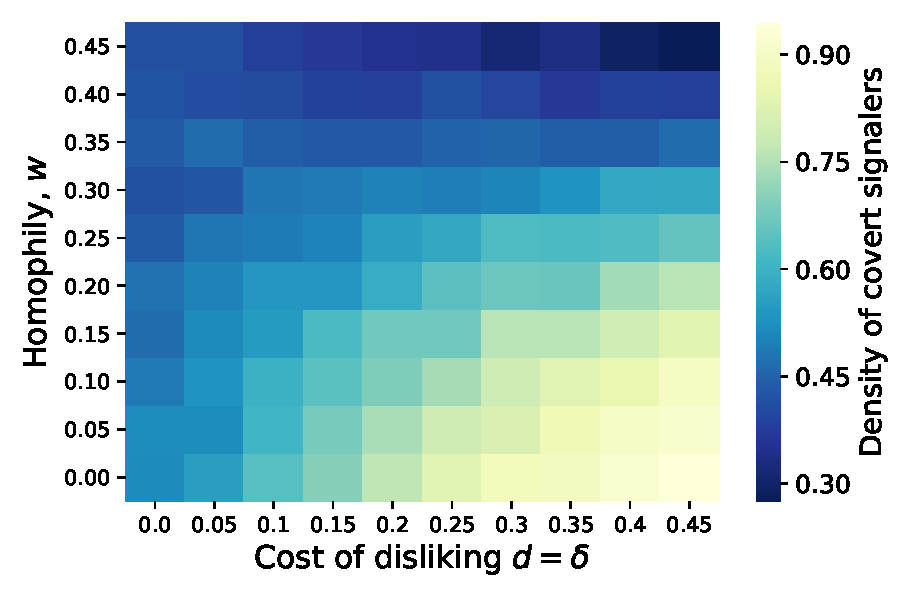
\includegraphics[width=\textwidth]{Figures/covertDensityVsDislikingHomophilyCoevo.pdf}
    \caption{Density of covert signalers.}
  \end{subfigure}
  \begin{subfigure}{0.49\textwidth}
    \centering
    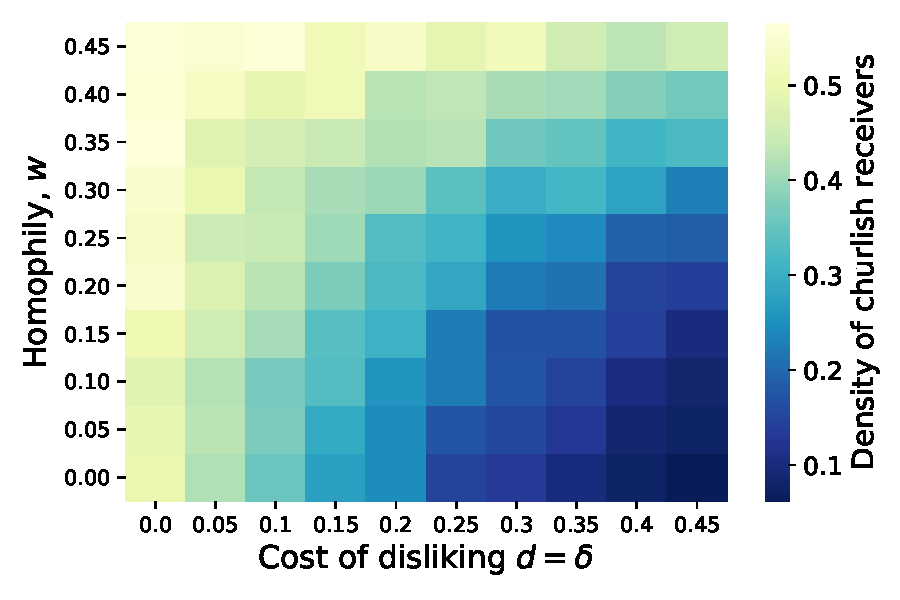
\includegraphics[width=\textwidth]{Figures/churlishDensityVsDislikingHomophilyCoevo.pdf}
    \caption{Density of churlish receivers.}
  \end{subfigure}
  
  \caption{Density of covert signalers and churlish receivers at $t=200$, 
    final timestep recorded in this preliminary experiment.}
  \label{fig:dislikingHomophilyHeatmap}
\end{figure}


\subsection{Correlations between proportion of covert signalers and of churlish receivers}

\begin{figure}[H]
  \centering
  \begin{subfigure}{0.49\textwidth}
    \centering
    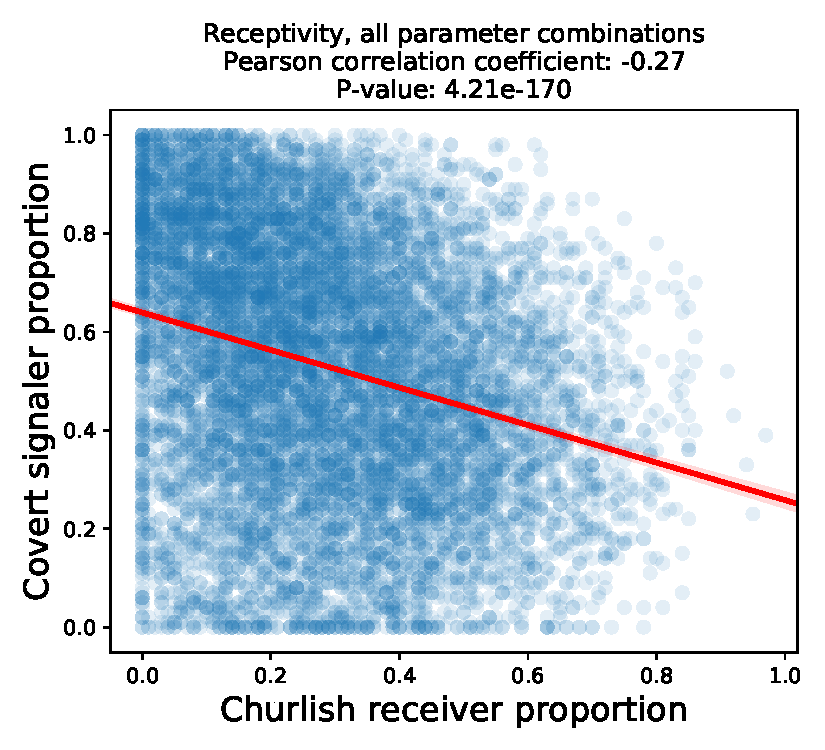
\includegraphics[width=\textwidth]{Figures/receptivity_allcombos_reg.pdf}
    \caption{}
    \label{fig:}
  \end{subfigure}
  \begin{subfigure}{0.49\textwidth}
    \centering
    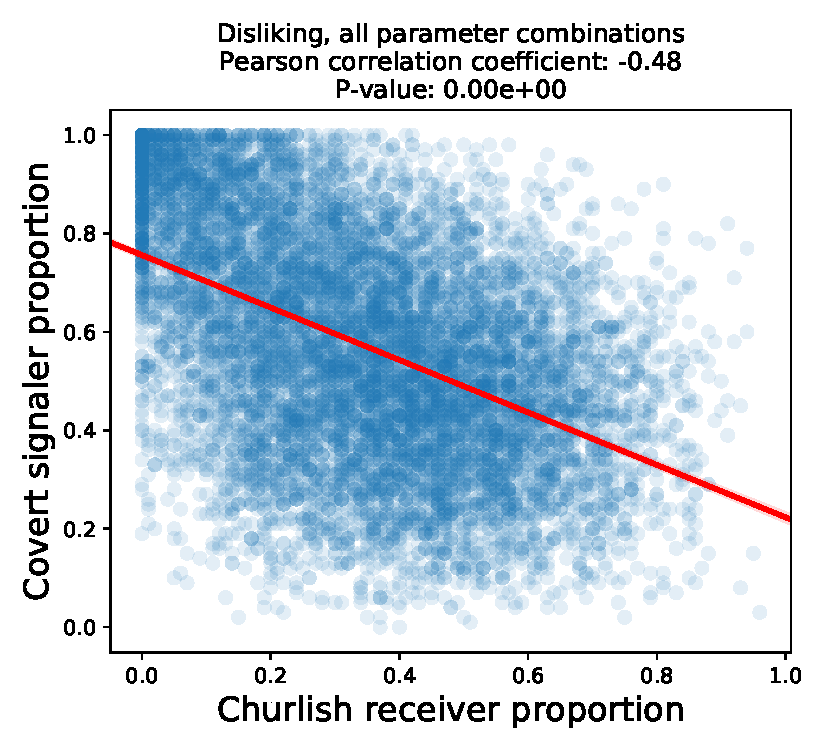
\includegraphics[width=\textwidth]{Figures/disliking_allcombos_reg.pdf}
    \caption{}
    \label{fig:}
  \end{subfigure}
  \caption{Correlation between proportion of covert signalers and proportion of
    churlish receivers for all tested parameter combinations in both 
    receptivity (a) and disliking (b) experiments.}
  \label{fig:regressions}
\end{figure}


\section{Invasion experiments}

Here we run identical experiments, but vary the initial proportion of 
churlish receivers and covert receivers over $\{0.05, 0.5, 0.95\}$ for a total
of nine parameter combinations. One of these is a repeat of the previous
experiments, where both parameters are set to 0.5. Below are two figures.
The first is nine parameter settings where the density of covert signalers
is plotted in a heatmap (Figure~\ref{fig:invasion-signaling}). The second has 
heatmaps of the density of churlish receivers (Figure~\ref{fig:invasion-receiving}).

\input{invasion-figures.tex}



\section{Minority populations}

So far in these results I tested the case where a 10\% or 25\% of all agents have
the minority trait, $+1$ in the first trait vector position. 
The other 90\% or 75\% have the majority trait, $-1$ in the first trait vector position.

$r=0.25$, $R=0.5$.

\subsection{Covert signaling}

\subsubsection{Fraction of minorities = 0.10}
\begin{figure}[H]
  \centering
  \begin{subfigure}{0.49\textwidth}
    \centering
    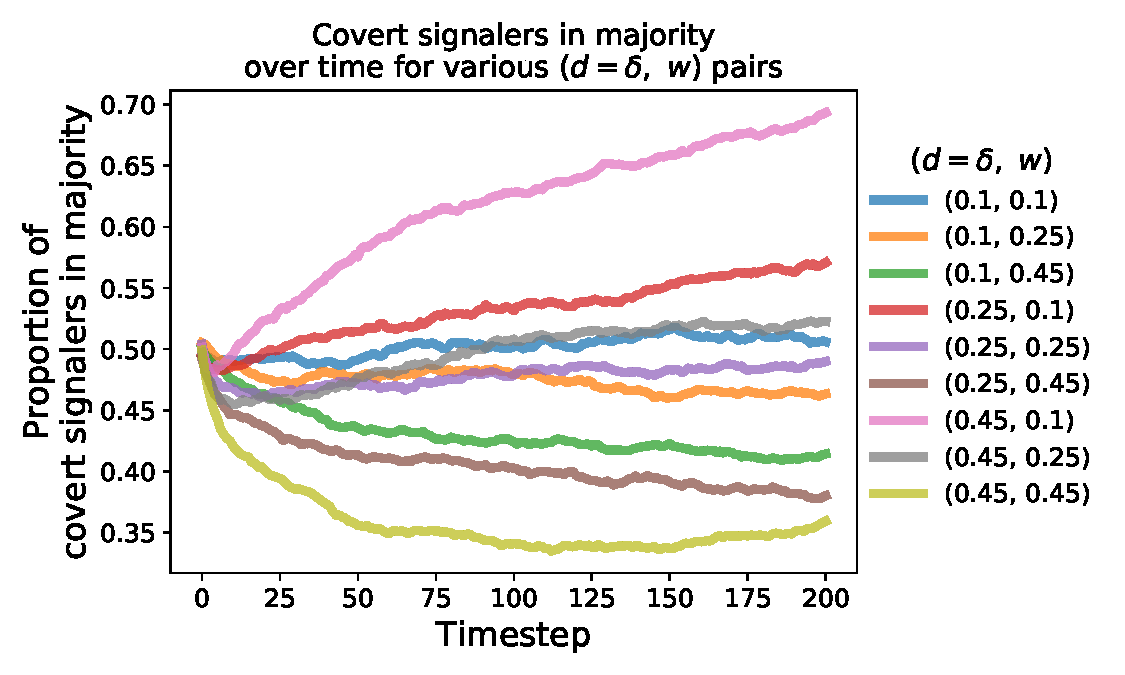
\includegraphics[width=\textwidth]{Figures/covert_series_majority.pdf}
    \caption{}
    \label{fig:}
  \end{subfigure}
  \begin{subfigure}{0.49\textwidth}
    \centering
    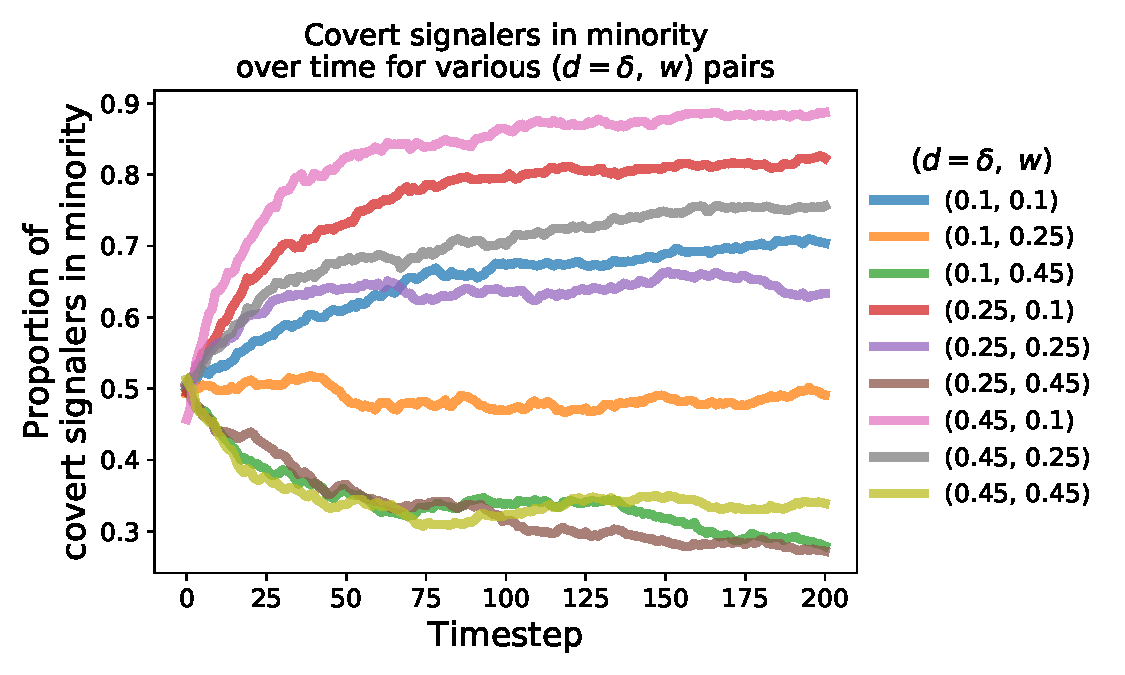
\includegraphics[width=\textwidth]{Figures/covert_series_minority.pdf}
    \caption{}
    \label{fig:}
  \end{subfigure}
  \caption{Mean timeseries of the evolution of covert signaling in the
    majority (a) and minority (b) populations.}
  \label{fig:}
\end{figure}


\begin{figure}[H]
  \centering
  \begin{subfigure}{0.49\textwidth}
    \centering
    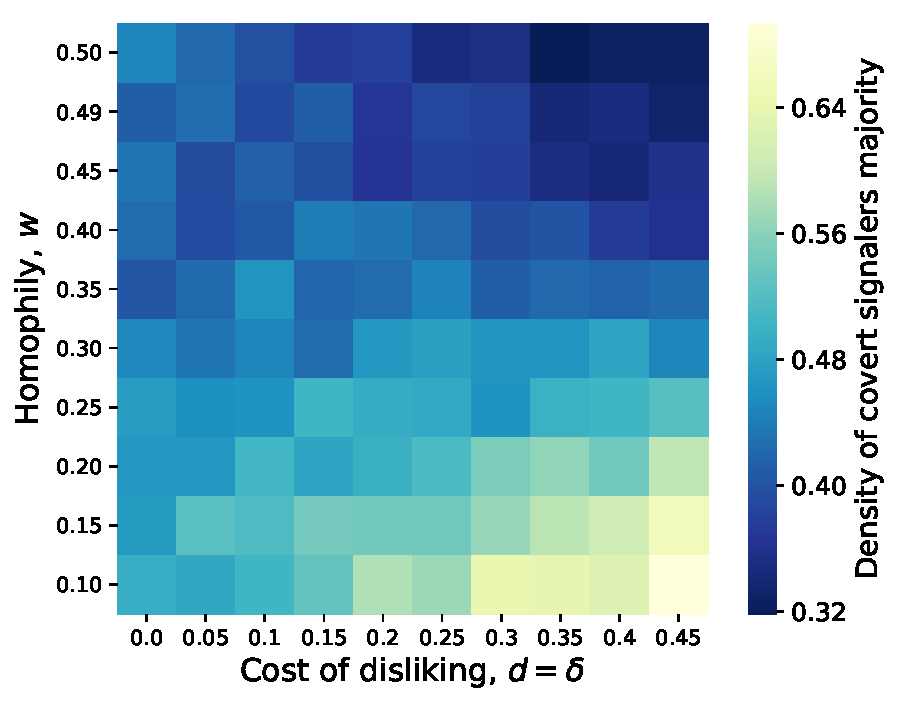
\includegraphics[width=\textwidth]{Figures/majority_signalers.pdf}
    \caption{}
    \label{fig:}
  \end{subfigure}
  \begin{subfigure}{0.49\textwidth}
    \centering
    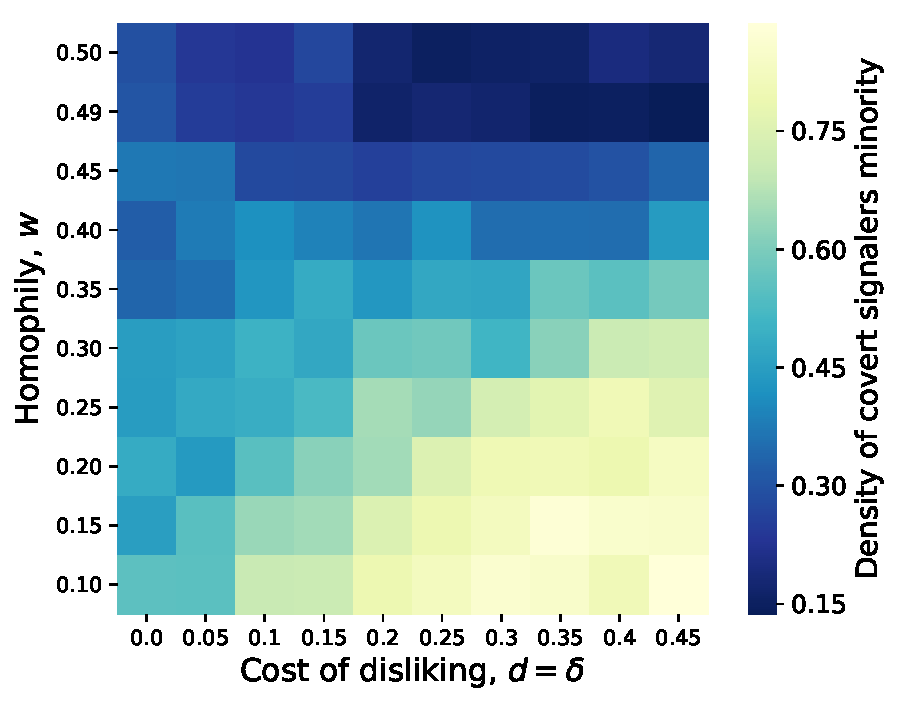
\includegraphics[width=\textwidth]{Figures/minority_signalers.pdf}
    \caption{}
    \label{fig:}
  \end{subfigure}
  \caption{Proprtion of covert signalers for different parameter settings in the
    majority (a) and minority (b) populations.}
  \label{fig:regressions}
\end{figure}

\begin{figure}[H]
  \centering
    \includegraphics[width=0.6\textwidth]{Figures/covert_signalers_diff.pdf}
  \caption{Difference between proportion of covert signalers in the minority 
    and majority populations. When cost of disliking is high and homophily is 
    low, more minority agents are covert signalers than majority agents,
    proportionally. An increase in homophily enables minority agents to 
    find one another more easily, so overt signaling, which reaches more of
    the population, is advantageous.
  }
  \label{fig:}
\end{figure}

\subsubsection{Fraction of minorities = 0.25}

\begin{figure}[H]
  \centering
  \begin{subfigure}{0.49\textwidth}
    \centering
    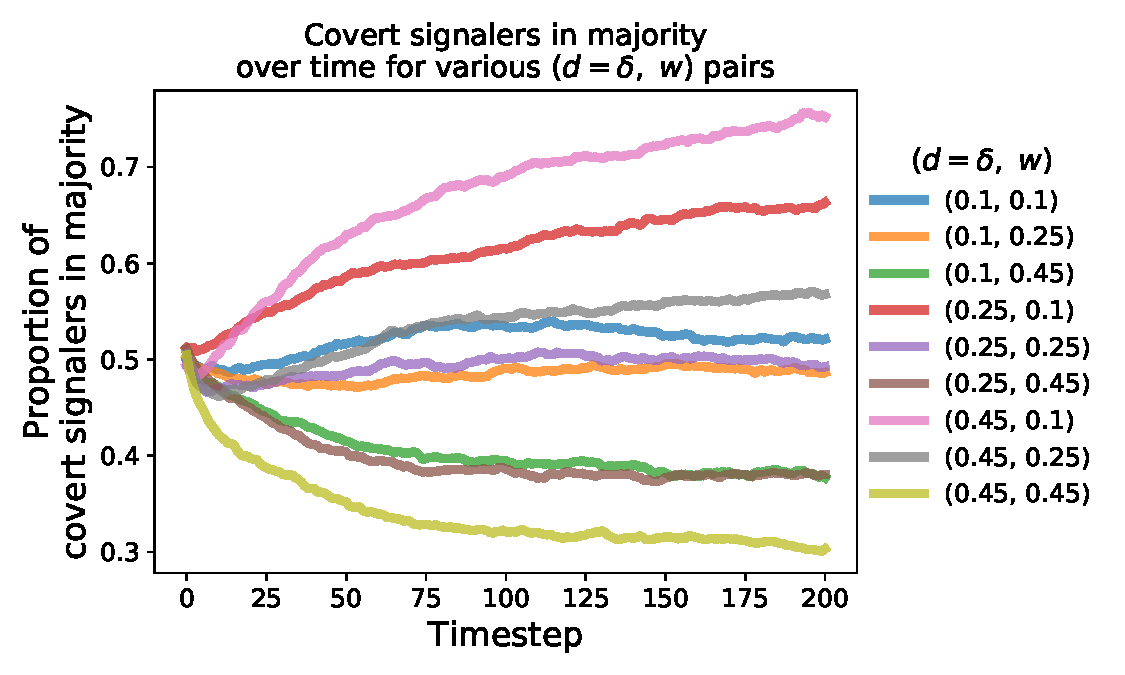
\includegraphics[width=\textwidth]{Figures/covert_series_majority_025.pdf}
    \caption{}
    \label{fig:}
  \end{subfigure}
  \begin{subfigure}{0.49\textwidth}
    \centering
    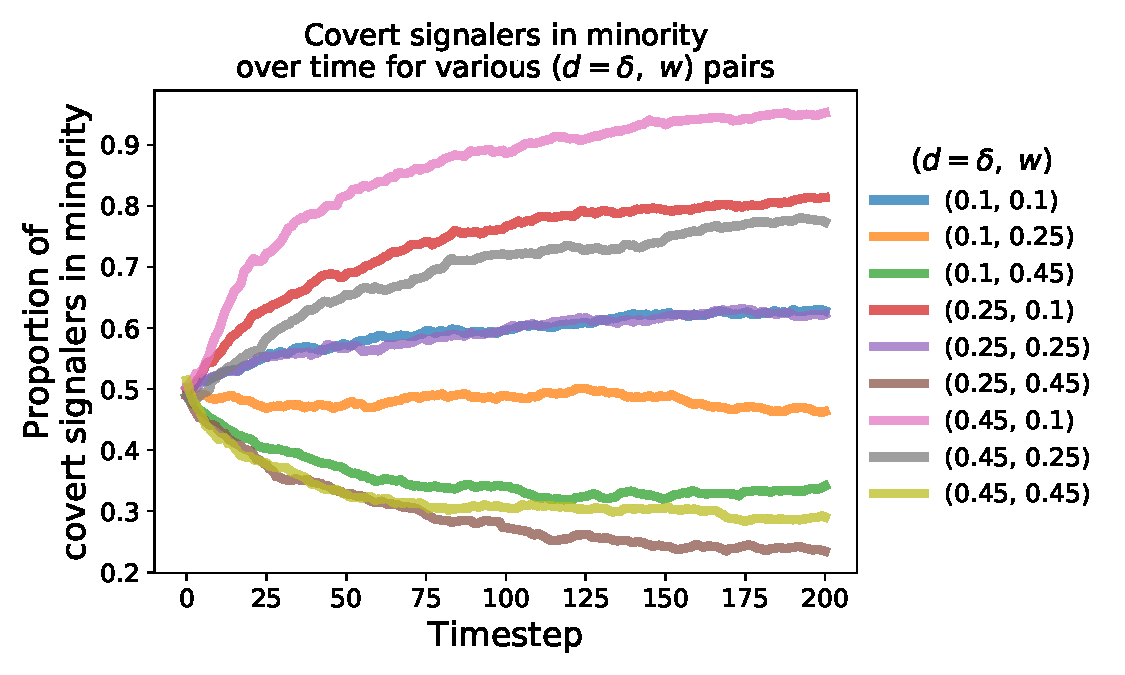
\includegraphics[width=\textwidth]{Figures/covert_series_minority_025.pdf}
    \caption{}
    \label{fig:}
  \end{subfigure}
  \caption{Mean timeseries of the evolution of covert signaling in the
    majority (a) and minority (b) populations.}
  \label{fig:regressions}
\end{figure}


\begin{figure}[H]
  \centering
  \begin{subfigure}{0.49\textwidth}
    \centering
    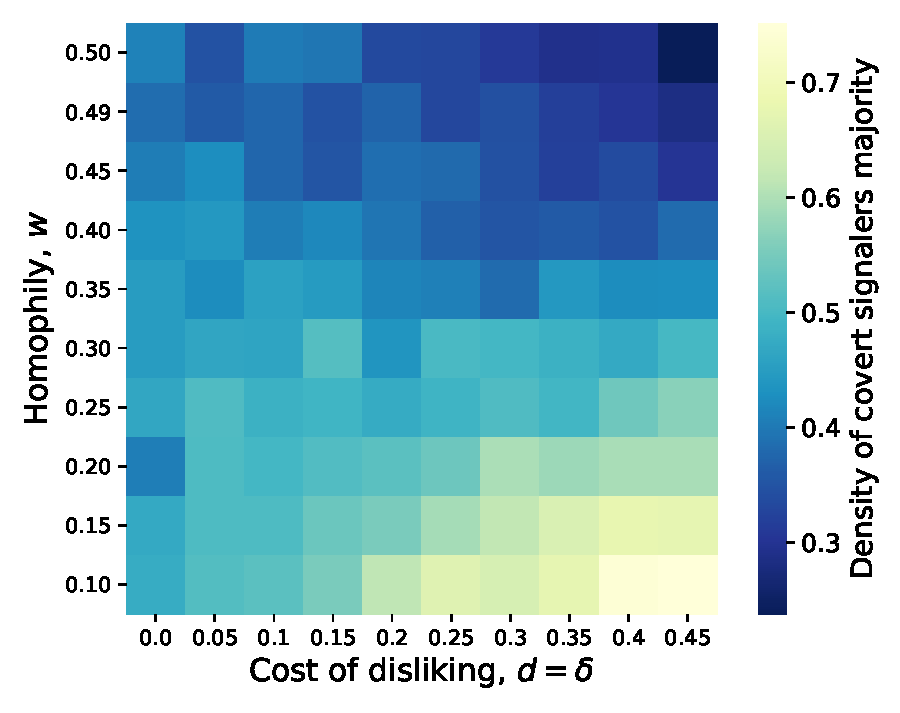
\includegraphics[width=\textwidth]{Figures/majority_signalers_025.pdf}
    \caption{}
    \label{fig:}
  \end{subfigure}
  \begin{subfigure}{0.49\textwidth}
    \centering
    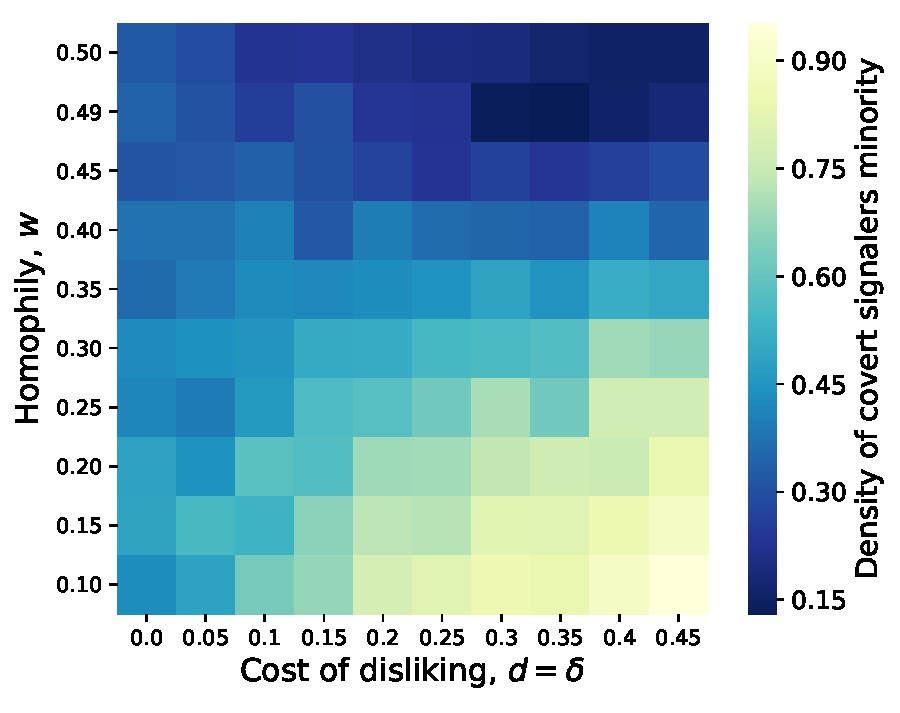
\includegraphics[width=\textwidth]{Figures/minority_signalers_025.pdf}
    \caption{}
    \label{fig:}
  \end{subfigure}
  \caption{Proprtion of covert signalers for different parameter settings in the
    majority (a) and minority (b) populations.}
  \label{fig:regressions}
\end{figure}

\begin{figure}[H]
  \centering
    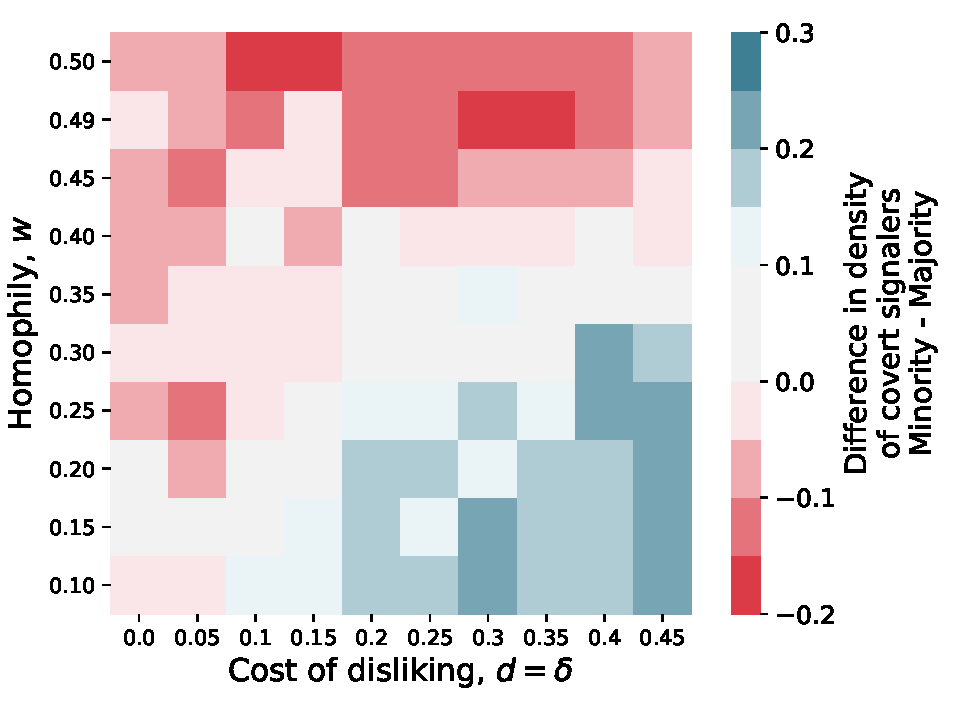
\includegraphics[width=0.6\textwidth]{Figures/covert_signalers_diff_025.pdf}
  \caption{Difference between proportion of covert signalers in the minority 
    and majority populations. When cost of disliking is high and homophily is 
    low, more minority agents are covert signalers than majority agents,
    proportionally. An increase in homophily enables minority agents to 
    find one another more easily, so overt signaling, which reaches more of
    the population, is advantageous.
  }
  \label{fig:}
\end{figure}

\subsubsection{Fraction of minorities = 0.05}

\begin{figure}[H]
  \centering
  \begin{subfigure}{0.49\textwidth}
    \centering
    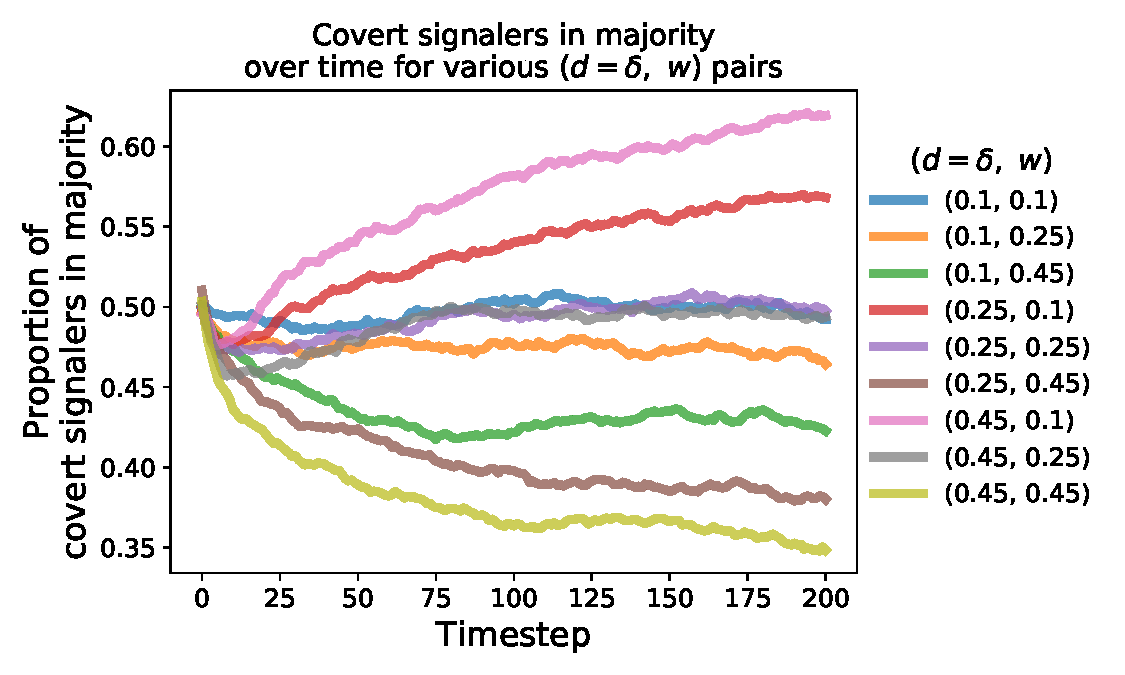
\includegraphics[width=\textwidth]{Figures/covert_series_majority_005.pdf}
    \caption{}
    \label{fig:}
  \end{subfigure}
  \begin{subfigure}{0.49\textwidth}
    \centering
    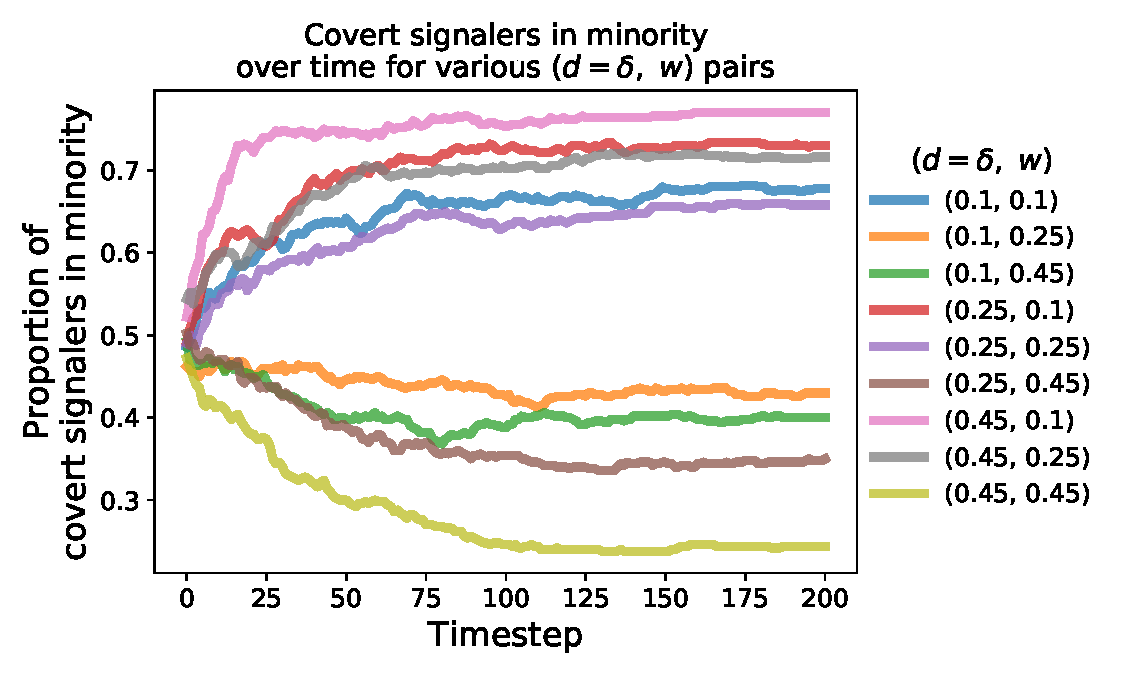
\includegraphics[width=\textwidth]{Figures/covert_series_minority_005.pdf}
    \caption{}
    \label{fig:}
  \end{subfigure}
  \caption{Mean timeseries of the evolution of covert signaling in the
    majority (a) and minority (b) populations.}
  \label{fig:regressions}
\end{figure}


\begin{figure}[H]
  \centering
  \begin{subfigure}{0.49\textwidth}
    \centering
    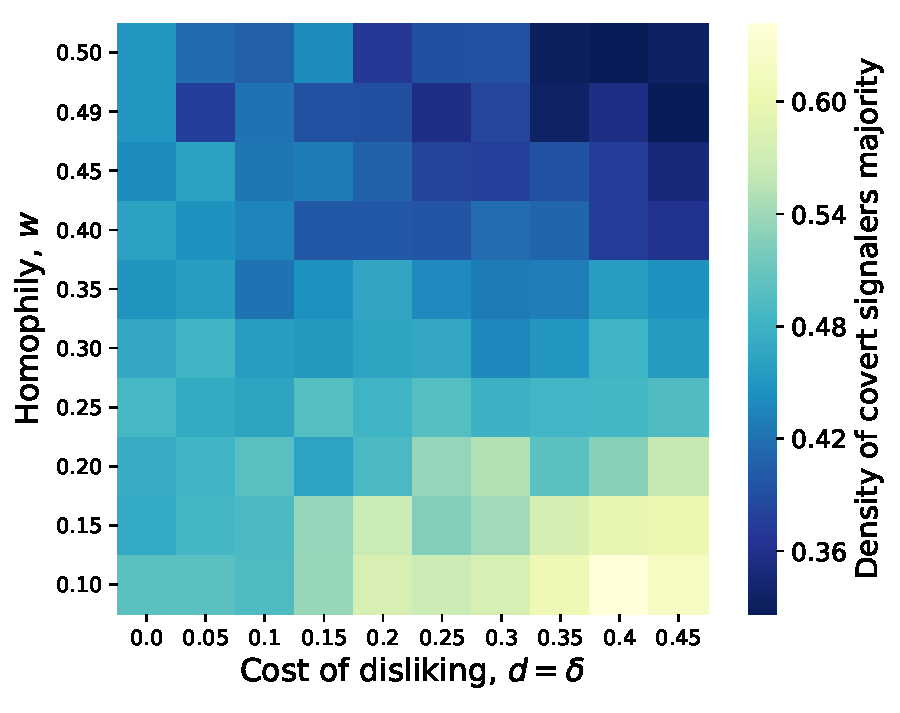
\includegraphics[width=\textwidth]{Figures/majority_signalers_005.pdf}
    \caption{}
    \label{fig:}
  \end{subfigure}
  \begin{subfigure}{0.49\textwidth}
    \centering
    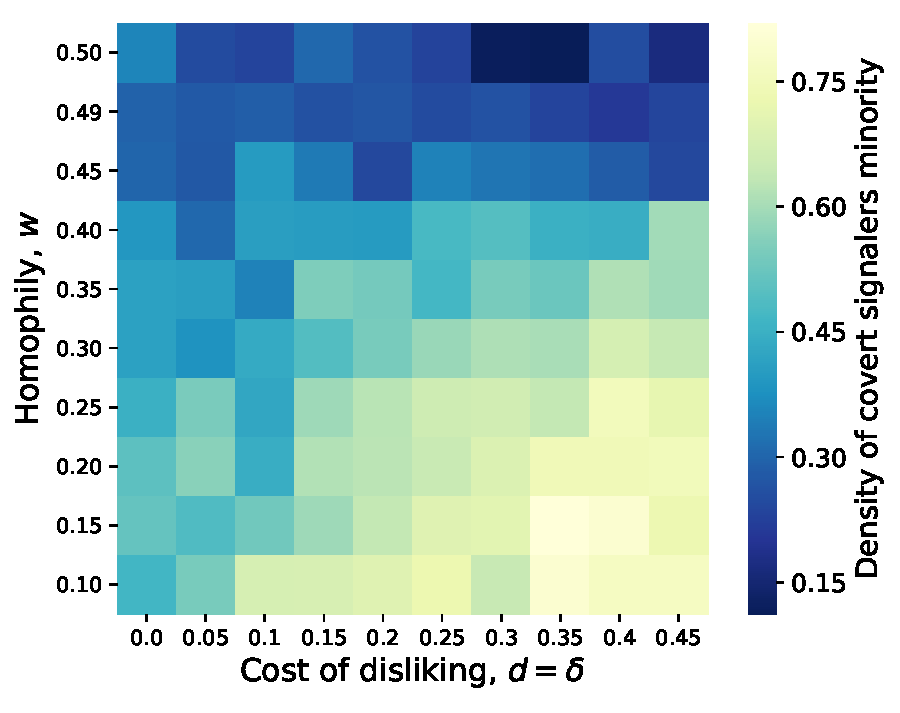
\includegraphics[width=\textwidth]{Figures/minority_signalers_005.pdf}
    \caption{}
    \label{fig:}
  \end{subfigure}
  \caption{Proprtion of covert signalers for different parameter settings in the
    majority (a) and minority (b) populations.}
  \label{fig:regressions}
\end{figure}

\begin{figure}[H]
  \centering
    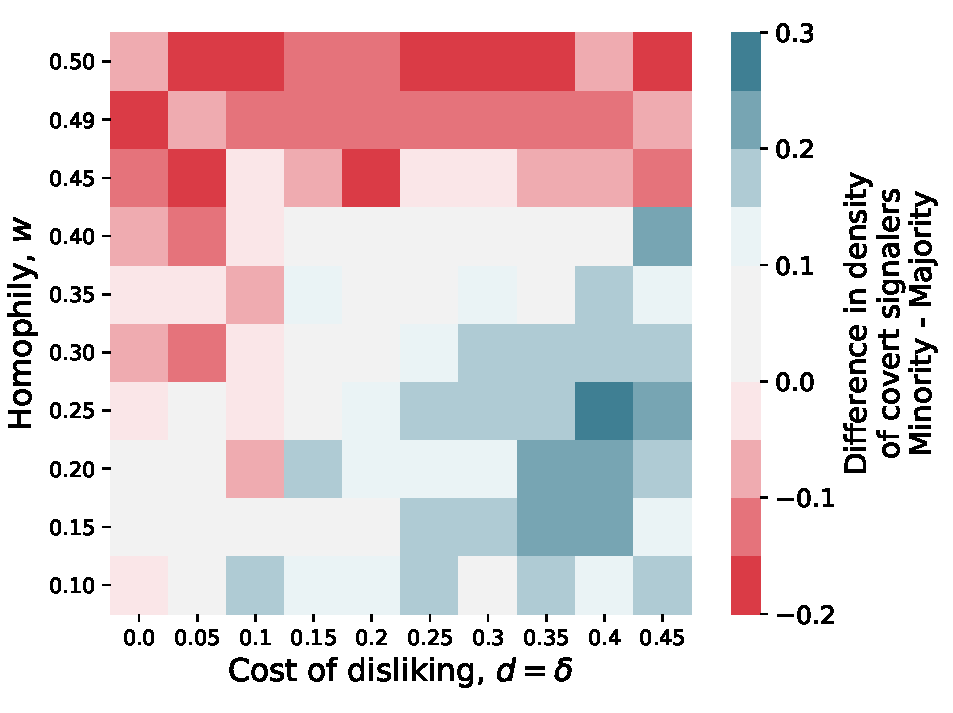
\includegraphics[width=0.6\textwidth]{Figures/covert_signalers_diff_005.pdf}
  \caption{Difference between proportion of covert signalers in the minority 
    and majority populations. When cost of disliking is high and homophily is 
    low, more minority agents are covert signalers than majority agents,
    proportionally. An increase in homophily enables minority agents to 
    find one another more easily, so overt signaling, which reaches more of
    the population, is advantageous.
  }
  \label{fig:}
\end{figure}


\subsection{Churlish receiving}

\subsubsection{Fraction of minorities = 0.10}

\begin{figure}[H]
  \centering
  \begin{subfigure}{0.49\textwidth}
    \centering
    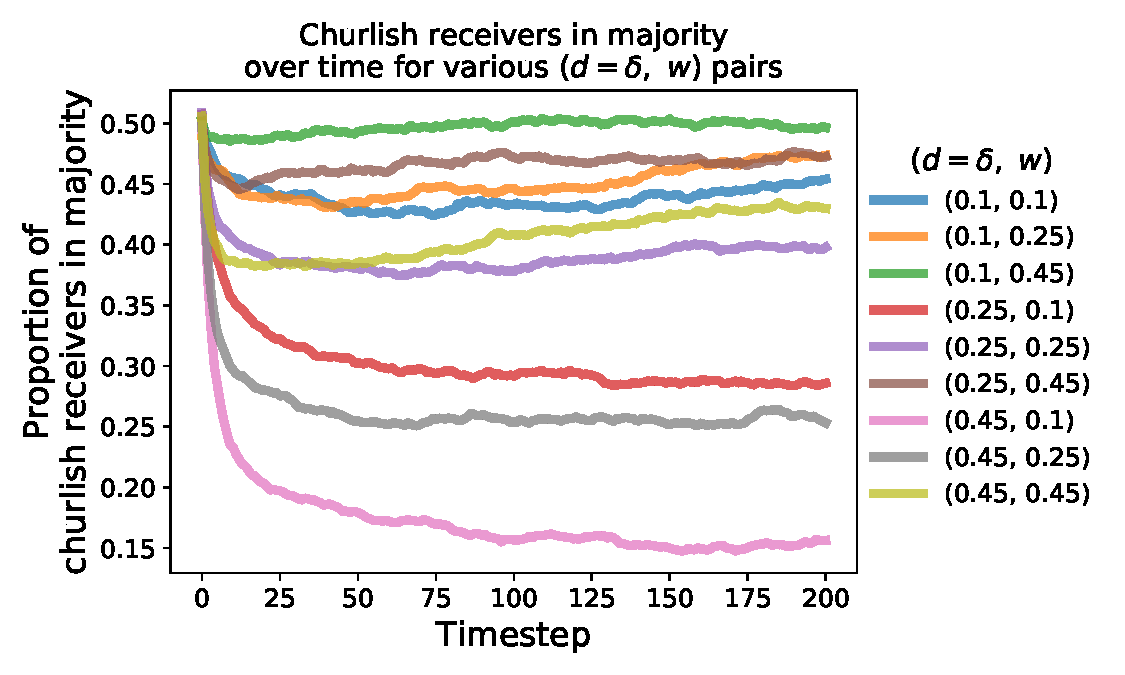
\includegraphics[width=\textwidth]{Figures/churlish_series_majority.pdf}
    \caption{}
    \label{fig:}
  \end{subfigure}
  \begin{subfigure}{0.49\textwidth}
    \centering
    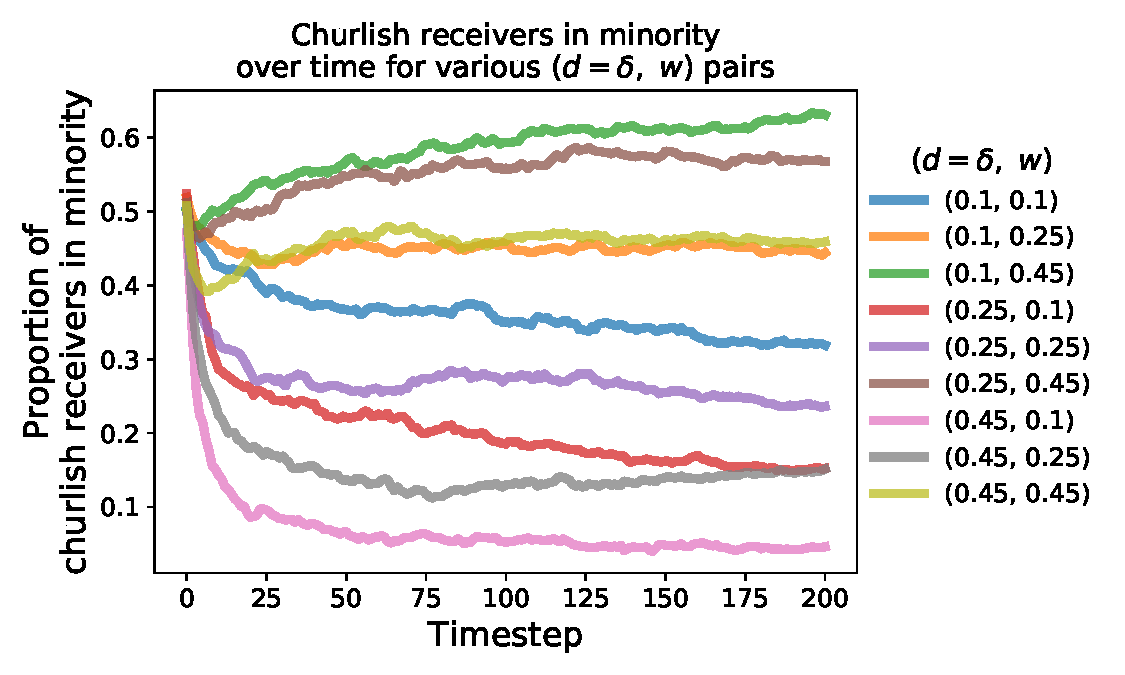
\includegraphics[width=\textwidth]{Figures/churlish_series_minority.pdf}
    \caption{}
    \label{fig:}
  \end{subfigure}
  \caption{Mean timeseries of the evolution of churlish receiving in the
    majority (a) and minority (b) populations.}
  \label{fig:regressions}
\end{figure}


\begin{figure}[H]
  \centering
  \begin{subfigure}{0.49\textwidth}
    \centering
    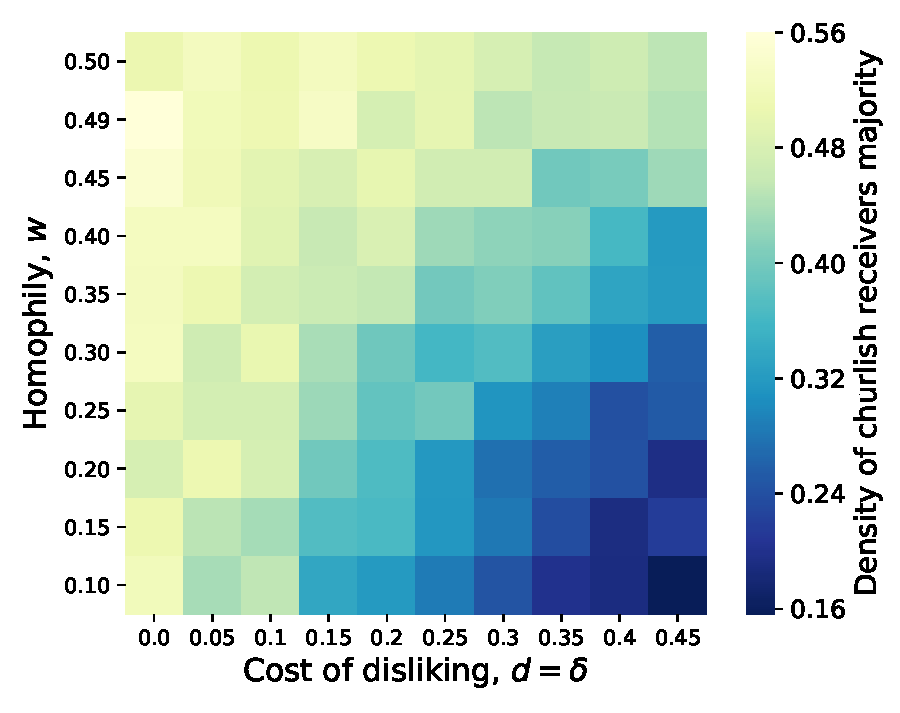
\includegraphics[width=\textwidth]{Figures/majority_receivers.pdf}
    \caption{}
    \label{fig:}
  \end{subfigure}
  \begin{subfigure}{0.49\textwidth}
    \centering
    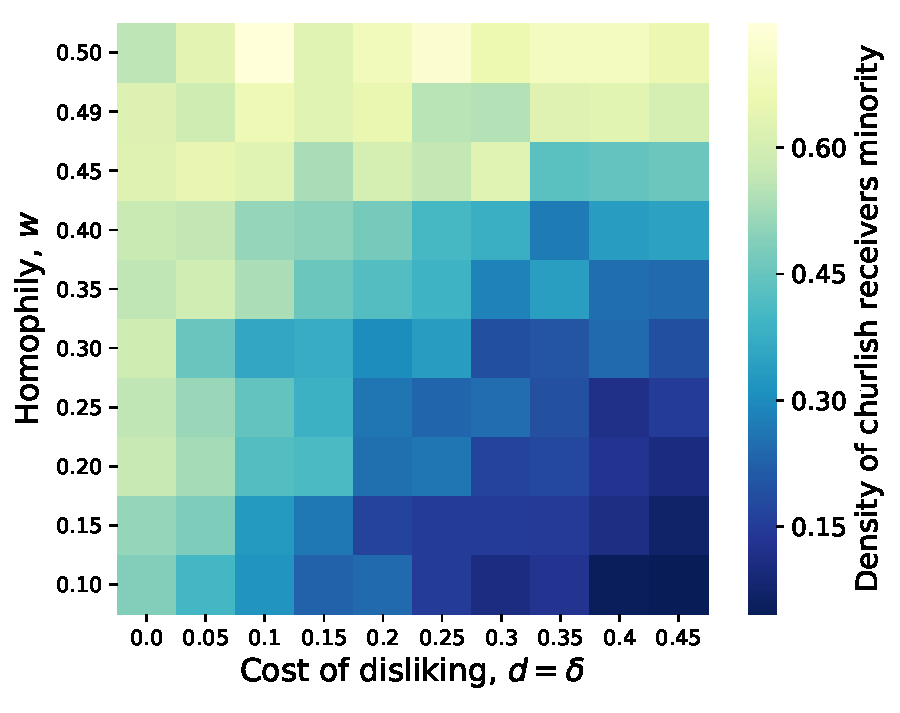
\includegraphics[width=\textwidth]{Figures/minority_receivers.pdf}
    \caption{}
    \label{fig:}
  \end{subfigure}
  \caption{Proprtion of churlish receivers for different parameter settings in the
    majority (a) and minority (b) populations.}
  \label{fig:regressions}
\end{figure}

\begin{figure}[H]
  \centering
    \includegraphics[width=0.6\textwidth]{Figures/churlish_receivers_diff.pdf}
  \caption{Difference between proportion of churlish receivers in the minority 
    and majority populations. Here the dependence is primarily on homophily.
    If homophily is too low, the minority population cannot interact often
    enough with their in-group, and so must adopt a non-churlish stance towards
    others in order to not suffer cost of disliking penalties. Once the minority
    can reliably find its in-group members (increasing homophily) the minority
    can afford to assume they dislike others, since by and large they dislike
    the majority.
  }
  \label{fig:}
\end{figure}


\subsubsection{Fraction of minorities = 0.25}

\begin{figure}[H]
  \centering
  \begin{subfigure}{0.49\textwidth}
    \centering
    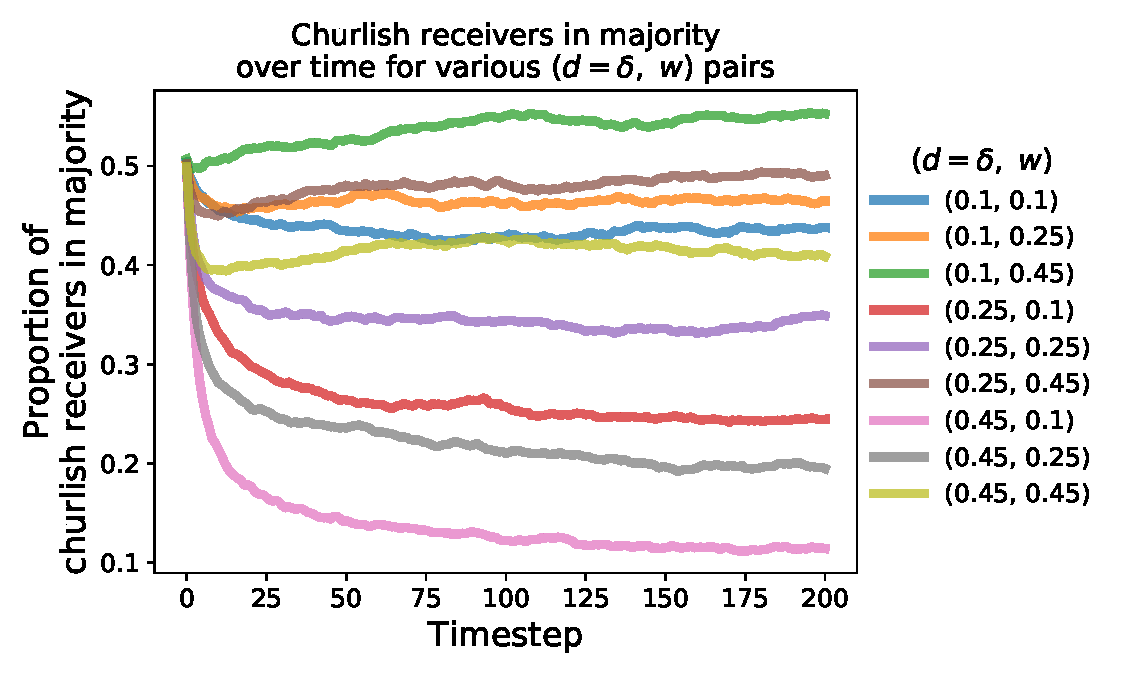
\includegraphics[width=\textwidth]{Figures/churlish_series_majority_025.pdf}
    \caption{}
    \label{fig:}
  \end{subfigure}
  \begin{subfigure}{0.49\textwidth}
    \centering
    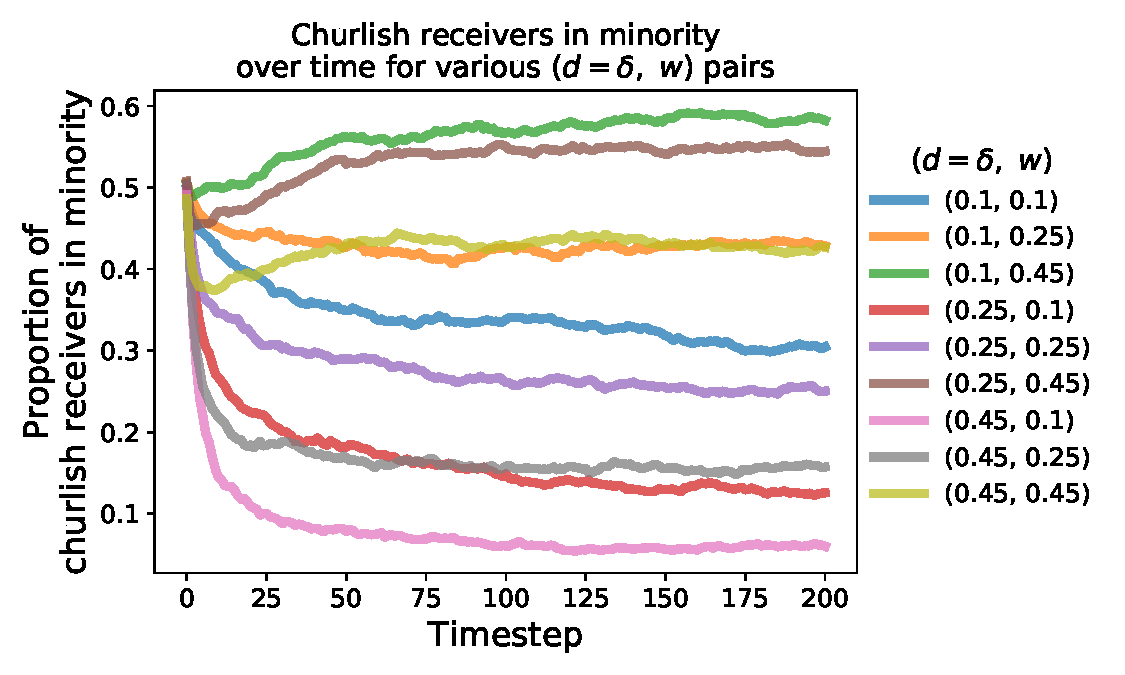
\includegraphics[width=\textwidth]{Figures/churlish_series_minority_025.pdf}
    \caption{}
    \label{fig:}
  \end{subfigure}
  \caption{Mean timeseries of the evolution of churlish receiving in the
    majority (a) and minority (b) populations.}
  \label{fig:regressions}
\end{figure}


\begin{figure}[H]
  \centering
  \begin{subfigure}{0.49\textwidth}
    \centering
    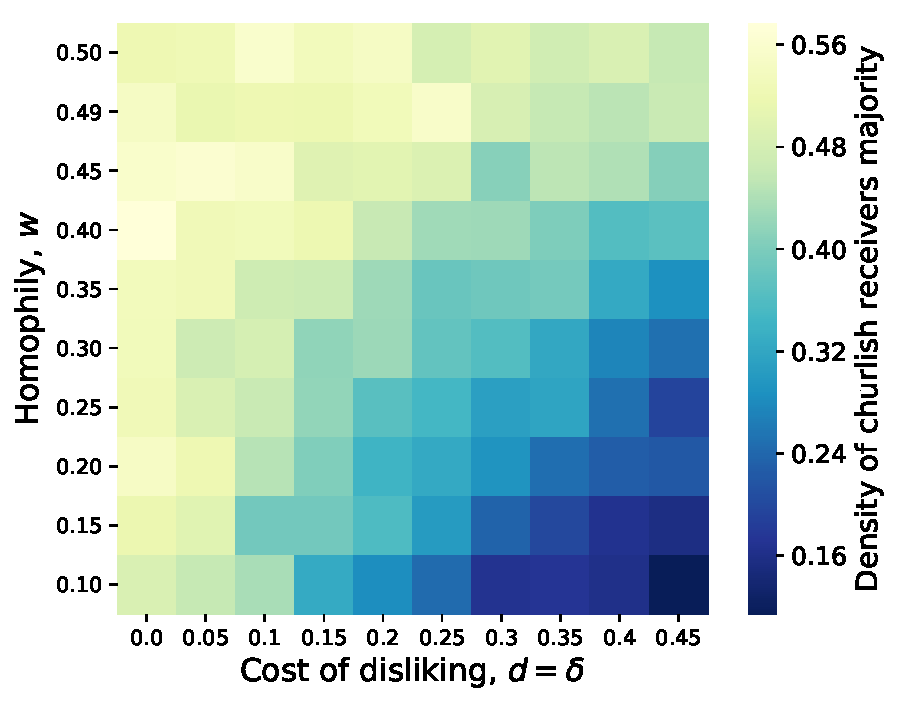
\includegraphics[width=\textwidth]{Figures/majority_receivers_025.pdf}
    \caption{}
    \label{fig:}
  \end{subfigure}
  \begin{subfigure}{0.49\textwidth}
    \centering
    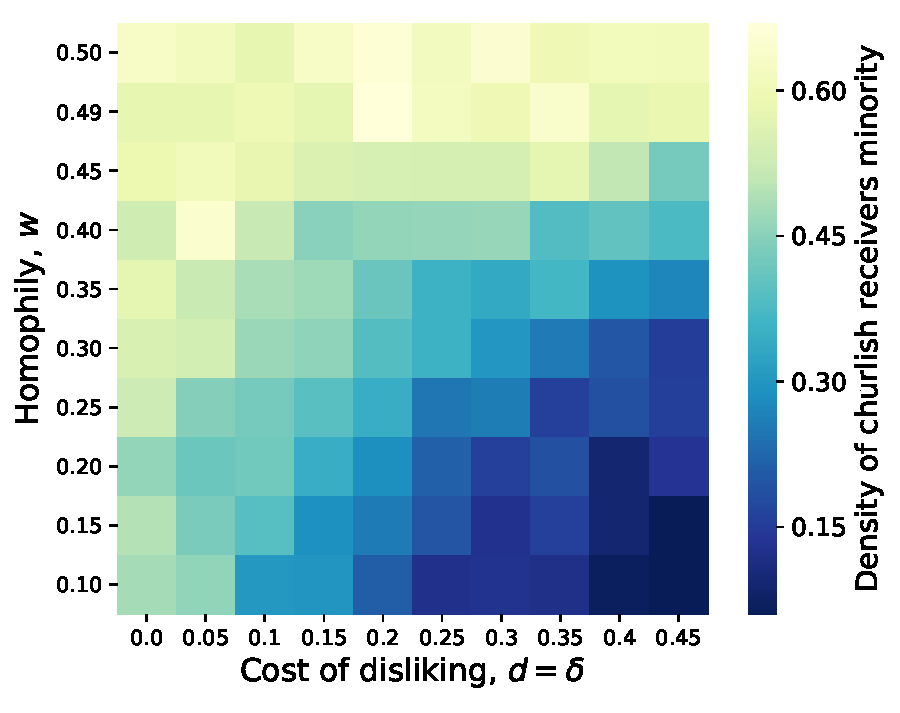
\includegraphics[width=\textwidth]{Figures/minority_receivers_025.pdf}
    \caption{}
    \label{fig:}
  \end{subfigure}
  \caption{Proprtion of churlish receivers for different parameter settings in the
    majority (a) and minority (b) populations.}
  \label{fig:regressions}
\end{figure}

\begin{figure}[H]
  \centering
    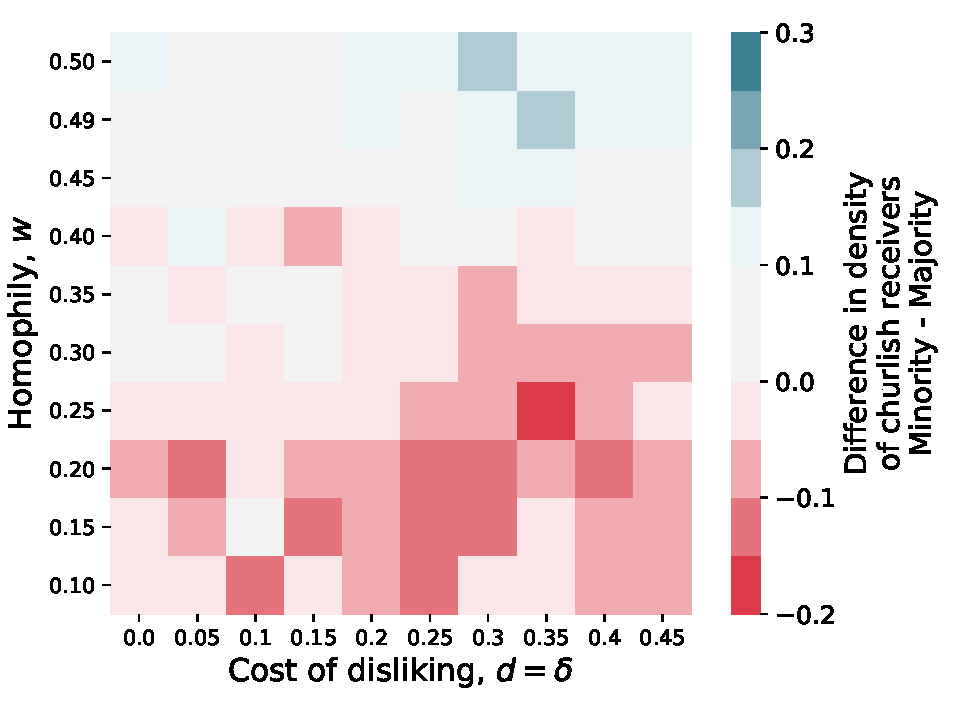
\includegraphics[width=0.6\textwidth]{Figures/churlish_receivers_diff_025.pdf}
  \caption{Difference between proportion of churlish receivers in the minority 
    and majority populations. Here the dependence is primarily on homophily.
    If homophily is too low, the minority population cannot interact often
    enough with their in-group, and so must adopt a non-churlish stance towards
    others in order to not suffer cost of disliking penalties. Once the minority
    can reliably find its in-group members (increasing homophily) the minority
    can afford to assume they dislike others, since by and large they dislike
    the majority.
  }
  \label{fig:}
\end{figure}


\subsubsection{Fraction of minorities = 0.05}

\begin{figure}[H]
  \centering
  \begin{subfigure}{0.49\textwidth}
    \centering
    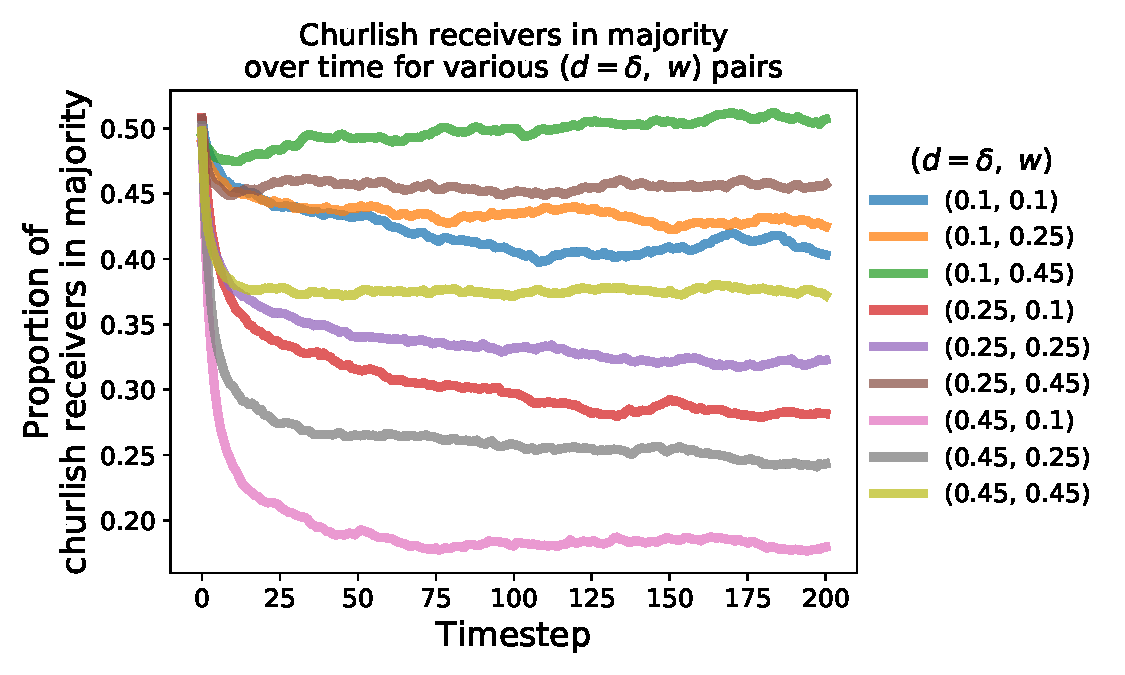
\includegraphics[width=\textwidth]{Figures/churlish_series_majority_005.pdf}
    \caption{}
    \label{fig:}
  \end{subfigure}
  \begin{subfigure}{0.49\textwidth}
    \centering
    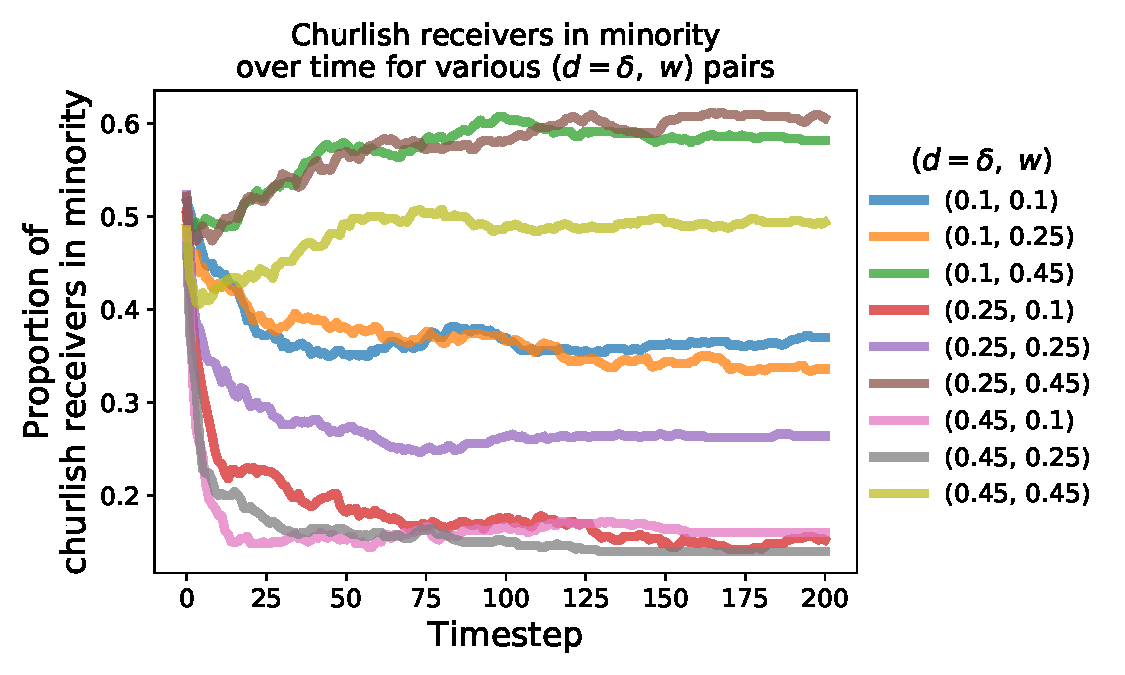
\includegraphics[width=\textwidth]{Figures/churlish_series_minority_005.pdf}
    \caption{}
    \label{fig:}
  \end{subfigure}
  \caption{Mean timeseries of the evolution of churlish receiving in the
    majority (a) and minority (b) populations.}
  \label{fig:regressions}
\end{figure}


\begin{figure}[H]
  \centering
  \begin{subfigure}{0.49\textwidth}
    \centering
    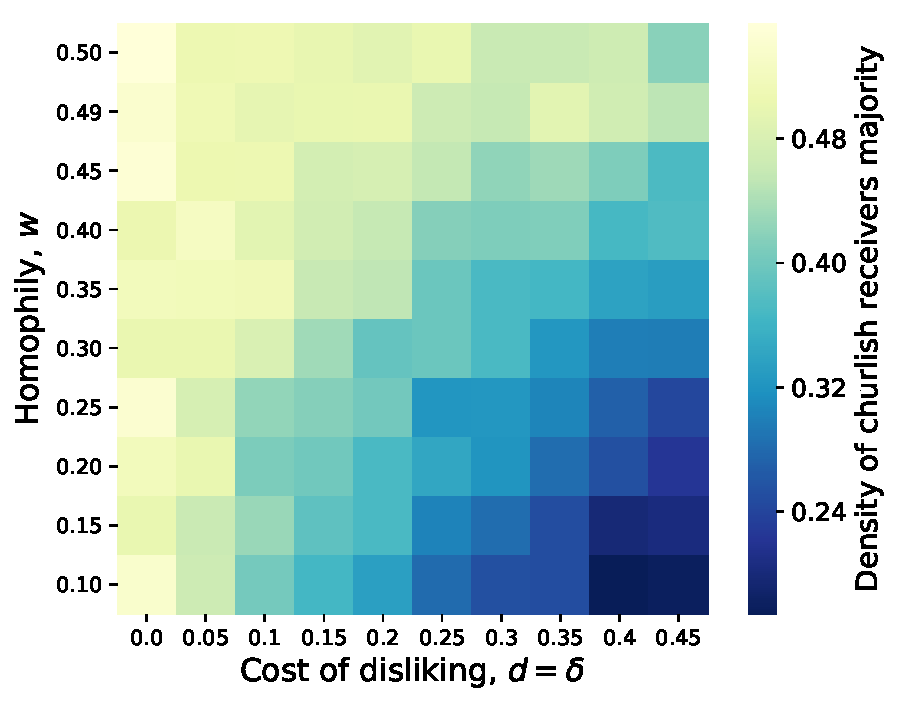
\includegraphics[width=\textwidth]{Figures/majority_receivers_005.pdf}
    \caption{}
    \label{fig:}
  \end{subfigure}
  \begin{subfigure}{0.49\textwidth}
    \centering
    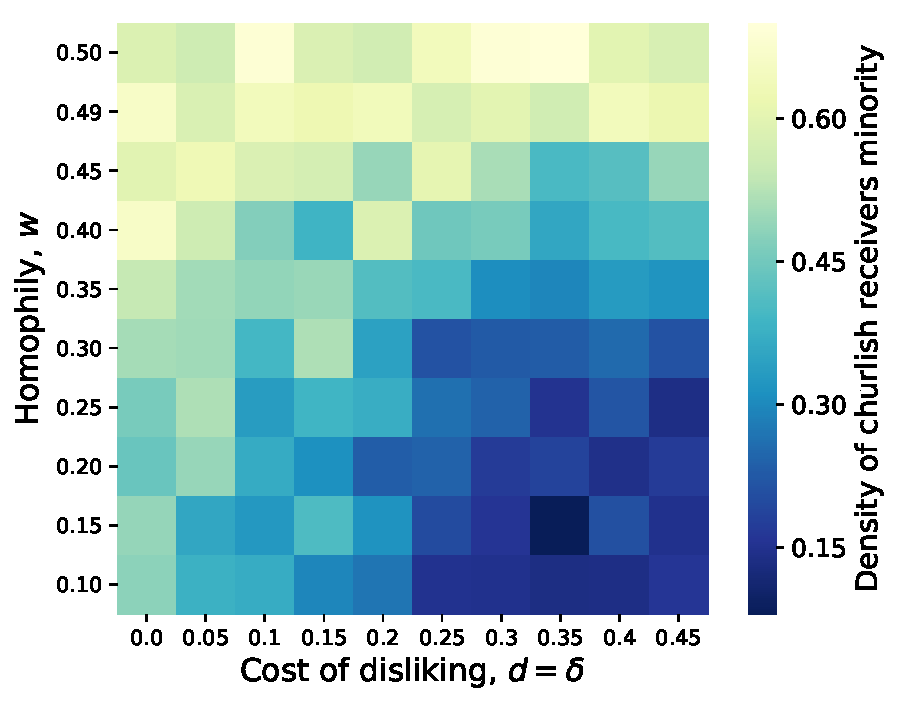
\includegraphics[width=\textwidth]{Figures/minority_receivers_005.pdf}
    \caption{}
    \label{fig:}
  \end{subfigure}
  \caption{Proprtion of churlish receivers for different parameter settings in the
    majority (a) and minority (b) populations.}
  \label{fig:regressions}
\end{figure}

\begin{figure}[H]
  \centering
    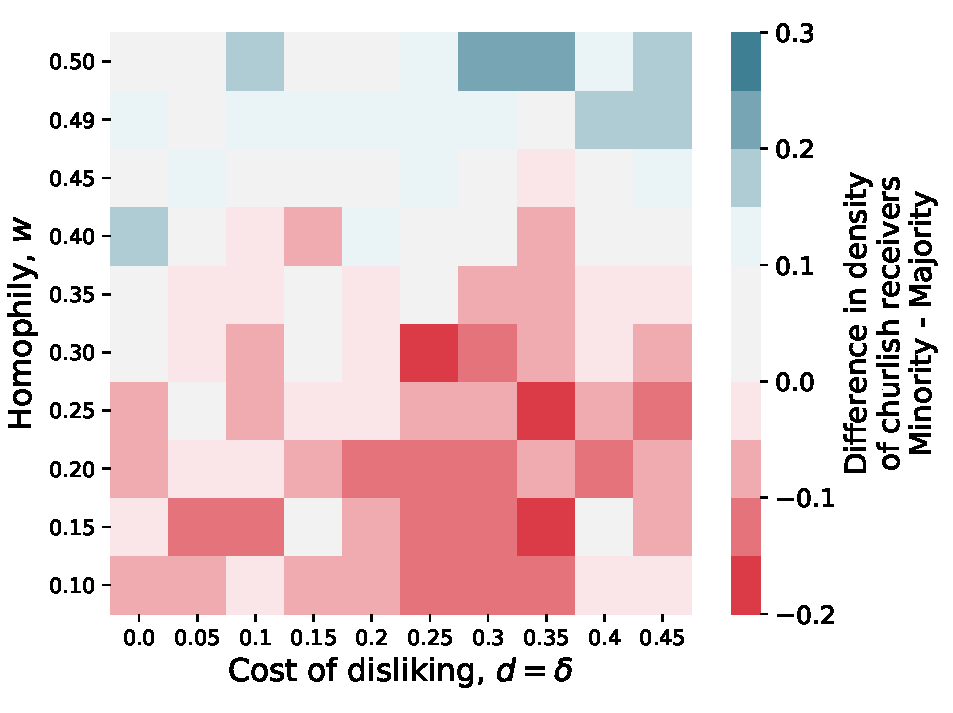
\includegraphics[width=0.6\textwidth]{Figures/churlish_receivers_diff_005.pdf}
  \caption{Difference between proportion of churlish receivers in the minority 
    and majority populations. Here the dependence is primarily on homophily.
    If homophily is too low, the minority population cannot interact often
    enough with their in-group, and so must adopt a non-churlish stance towards
    others in order to not suffer cost of disliking penalties. Once the minority
    can reliably find its in-group members (increasing homophily) the minority
    can afford to assume they dislike others, since by and large they dislike
    the majority.
  }
  \label{fig:}
\end{figure}


% \section{Discussion}

% These preliminary experiments and results are based on one major finding from
% ECS that covert signaling is maintained when overt signalers do not have
% too large an advantage in the free choice context. ``This requires that
% assortment with liked individuals not be too accurate,'' which corresponds to
% small $w$ in this ABM version. ``The accuracy of assortment is influenced
% by the reception probabilities of both signal types, $R$ and $r$'' (see p.
% 4 in ECS). Our preliminary results find the same trend with our ABM.


% \bibliographystyle{apacite}

% \setlength{\bibleftmargin}{.125in}
% \setlength{\bibindent}{-\bibleftmargin}

% \bibliography{/Users/mt/workspace/papers/library.bib}

\end{document}
